\documentclass[11pt]{article} % use larger type; default would be 10pt

\usepackage{pgfplots}
\usetikzlibrary{calc}
\usetikzlibrary{arrows}
\usetikzlibrary{patterns}
\usetikzlibrary{calc,intersections,through,backgrounds}
\usetikzlibrary{decorations.pathreplacing}
        \newcommand\degree[0]{^{\circ}}
        \newcommand\abs[1]{\left|#1\right|}

\title{Play with TikZ}
\author{Just Us}
%\date{} % Activate to display a given date or no date (if empty),
         % otherwise the current date is printed 

\begin{document}
\maketitle

\section{Chap 2 Section 1}



fig-2-1-1 number line

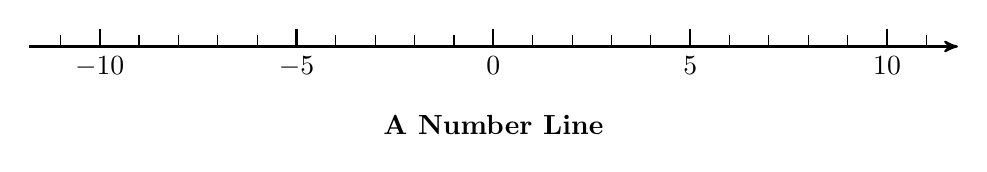
\begin{tikzpicture} [scale=0.5]
\draw[black,thick,->,>=stealth'] (-11.8,0) -- (11.8,0);
\foreach \x in  {-11, -10,...,11} {
 \draw[black] (\x,0.3) --++(0,-0.3);
}
\foreach \x in  {-10, -5, ..., 10} {
 \draw[black, thick] (\x,.45) --++(0,-0.45)  node[below]   {$\x$};
}
\node[below, ] at (0,-1.5) {\textbf{A Number Line}};
\end{tikzpicture}
\newline


fig-2-1-2 number line

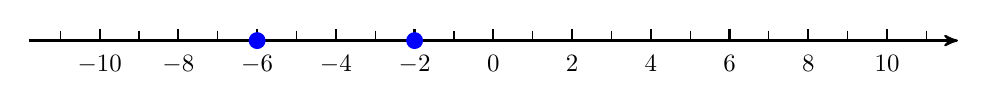
\begin{tikzpicture} [scale=0.5]
\draw[black,thick,->,>=stealth'] (-11.8,0) -- (11.8,0);
\foreach \x in  {-11, -10,...,11} {
 \draw[black] (\x,0.25) --++(0,-0.25);
}
\foreach \x in  {-10, -8, ..., 10} {
 \draw[black, thick] (\x,.3) --++(0,-0.3)  node[below, yshift=-2, scale=.9]   {$\x$};
}
\foreach \x in {-6,-2} {
 \filldraw[blue] (\x,0) circle (.2);
}
\end{tikzpicture}
\newline


fig-2-1-3 inequalities

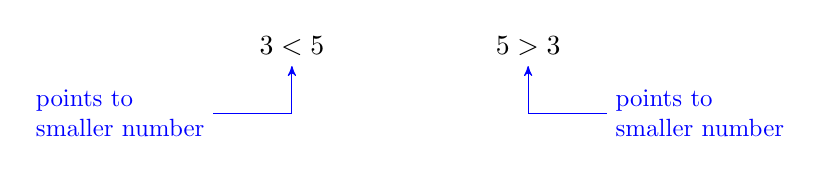
\begin{tikzpicture} 
\coordinate (O) at (0,0);
\node at (O) {$3 < 5$};
\draw[blue, <-, >=stealth'] (O)++(0,-.25)--++(0,-.6)--++(-1,0) node[left, scale=.9, align=left]{points to \\ smaller number};

\coordinate (O) at (3,0);
\node at (O) {$5 > 3$};
\draw[blue, <-, >=stealth'] (O)++(0,-.25)--++(0,-.6)--++(1,0) node[right, scale=.9, align=left]{points to \\ smaller number};
\end{tikzpicture}
\newline

fig-2-1-4 number line

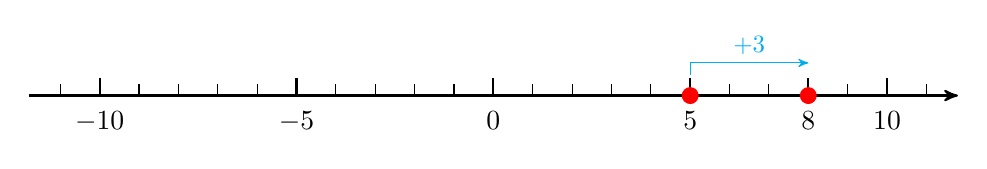
\begin{tikzpicture} [scale=0.5]
\draw[black,thick,->,>=stealth'] (-11.8,0) -- (11.8,0);
\foreach \x in  {-11, -10,...,11} {
 \draw[black] (\x,0.3) --++(0,-0.3);
}
\foreach \x in  {-10, -5, ..., 10,8} {
 \draw[black, thick] (\x,.45) --++(0,-0.45)  node[below, yshift=-2]   {$\x$};
}
\foreach \x in {5,8} {
 \filldraw[red] (\x,0) circle (.2);
}
\draw[cyan, ->, >=stealth'] (5,.53)--++(0,.3)--++(3,0) node[above, midway, scale=.9]{$+3$};
\end{tikzpicture}
\newline


fig-2-1-5 number line

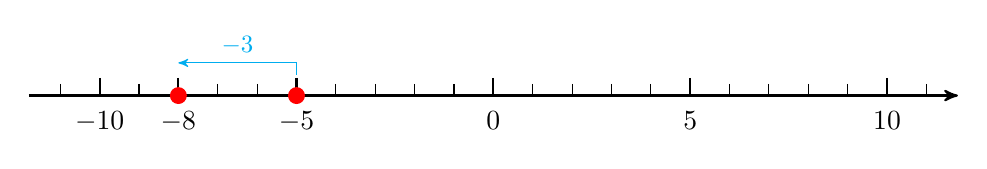
\begin{tikzpicture} [scale=0.5]
\draw[black,thick,->,>=stealth'] (-11.8,0) -- (11.8,0);
\foreach \x in  {-11, -10,...,11} {
 \draw[black] (\x,0.3) --++(0,-0.3);
}
\foreach \x in  {-10, -5, ..., 10,-8} {
 \draw[black, thick] (\x,.45) --++(0,-0.45)  node[below, yshift=-2]   {$\x$};
}
\foreach \x in {-5,-8} {
 \filldraw[red] (\x,0) circle (.2);
}
\draw[cyan, ->, >=stealth'] (-5,.53)--++(0,.3)--++(-3,0) node[above, midway, scale=.9]{$-3$};
\end{tikzpicture}
\newline


fig-2-1-6 number line

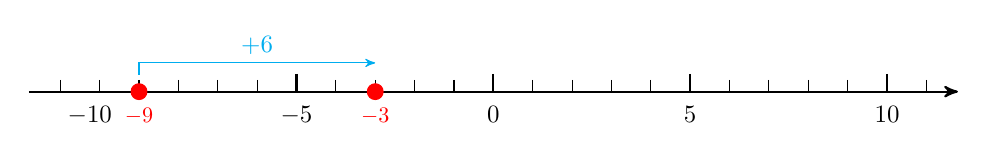
\begin{tikzpicture} [scale=0.5]
\draw[black,thick,->,>=stealth'] (-11.8,0) -- (11.8,0);
\foreach \x in  {-11, -10,...,11} {
 \draw[black] (\x,0.3) --++(0,-0.3);
}
\foreach \x in  { -5, 0,5, 10} {
 \draw[black, thick] (\x,.45) --++(0,-0.45)  node[below, yshift=-2, scale=.9]   {$\x$};
}
\node[below, yshift=-2, scale=.9] at (-10.25,0) {$-10$};
\foreach \x in {-9,-3} {
 \filldraw[red] (\x,0) circle (.2) node[below, yshift=-3, scale=.8] {$\x$};
}
\draw[cyan, ->, >=stealth'] (-9,.43)--++(0,.3)--++(6,0) node[above, midway, scale=.9]{$+6$};
\end{tikzpicture}
\newline


fig-2-1-7 number line

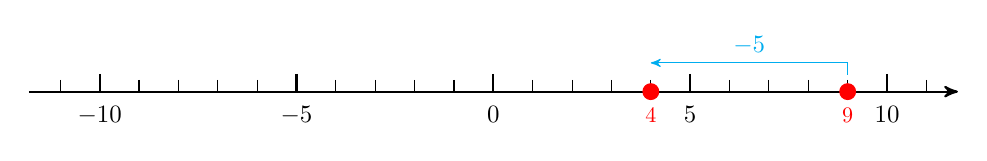
\begin{tikzpicture} [scale=0.5]
\draw[black,thick,->,>=stealth'] (-11.8,0) -- (11.8,0);
\foreach \x in  {-11, -10,...,11} {
 \draw[black] (\x,0.3) --++(0,-0.3);
}
\foreach \x in  {-10, -5, 0,5, 10} {
 \draw[black, thick] (\x,.45) --++(0,-0.45)  node[below, yshift=-2, scale=.9]   {$\x$};
}
\foreach \x in {4,9} {
 \filldraw[red] (\x,0) circle (.2) node[below, yshift=-3, scale=.8] {$\x$};
}
\draw[cyan, ->, >=stealth'] (9,.43)--++(0,.3)--++(-5,0) node[above, midway, scale=.9]{$-5$};
\end{tikzpicture}
\newline


fig-2-1-8 number line

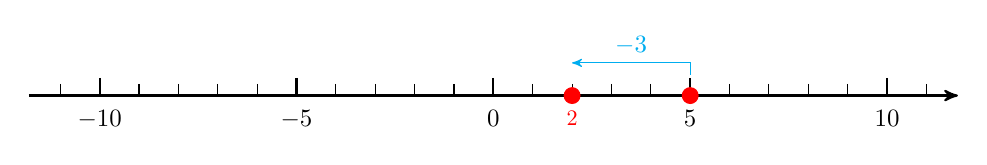
\begin{tikzpicture} [scale=0.5]
\draw[black,thick,->,>=stealth'] (-11.8,0) -- (11.8,0);
\foreach \x in  {-11, -10,...,11} {
 \draw[black] (\x,0.3) --++(0,-0.3);
}
\foreach \x in  {-10, -5, 0,5, 10} {
 \draw[black, thick] (\x,.45) --++(0,-0.45)  node[below, yshift=-2, scale=.9]   {$\x$};
}
\foreach \x in {2} {
 \filldraw[red] (\x,0) circle (.2) node[below, yshift=-3, scale=.8] {$\x$};
}
\filldraw[red] (5,0) circle (.2);
\draw[cyan, ->, >=stealth'] (5,.53)--++(0,.3)--++(-3,0) node[above, midway, scale=.9]{$-3$};
\end{tikzpicture}
\newline


fig-2-1-9 number line

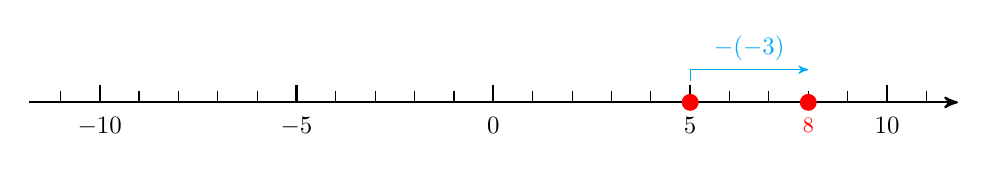
\begin{tikzpicture} [scale=0.5]
\draw[black,thick,->,>=stealth'] (-11.8,0) -- (11.8,0);
\foreach \x in  {-11, -10,...,11} {
 \draw[black] (\x,0.3) --++(0,-0.3);
}
\foreach \x in  {-10, -5, 0,5, 10} {
 \draw[black, thick] (\x,.45) --++(0,-0.45)  node[below, yshift=-2, scale=.9]   {$\x$};
}
\foreach \x in {8} {
 \filldraw[red] (\x,0) circle (.2) node[below, yshift=-3, scale=.8] {$\x$};
}
\filldraw[red] (5,0) circle (.2);
\draw[cyan, ->, >=stealth'] (5,.53)--++(0,.3)--++(3,0) node[above, midway, scale=.9]{$-(-3)$};
\end{tikzpicture}
\newline


fig-2-1-ex4a 3-10

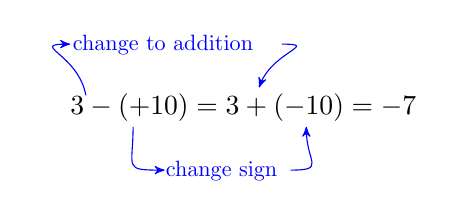
\begin{tikzpicture} 
\coordinate (O) at (0,0);
\node at (O) {$3 -(+10)=3+(-10)=-7$};
\coordinate(A) at (-2,0.15);
\coordinate(B) at (-2.2,.8);
\draw[blue, ->, >=stealth'] (A) to [out=100, in=180, looseness=2, edge node={node[above right, xshift=2, yshift=-3, scale=.8] {change to addition}}] (B);
\coordinate(A) at (0.49,0.8);
\coordinate(B) at (0.2,.25);
\draw[blue, ->, >=stealth'] (A) to [out=0, in=70, looseness=2] (B);
\coordinate(A) at (-1.4,-0.25);
\coordinate(B) at (-1.,-.8);
\draw[blue, ->, >=stealth'] (A) to [out=270, in=180, looseness=2, edge node={node[below right, xshift=9, yshift=4, scale=.8] {change sign}}] (B);
\coordinate(A) at (.6,-0.8);
\coordinate(B) at (.8,-.25);
\draw[blue, ->, >=stealth'] (A) to [out=0, in=270, looseness=2] (B);

\end{tikzpicture}
\newline


fig-2-1-ex4b -6-3

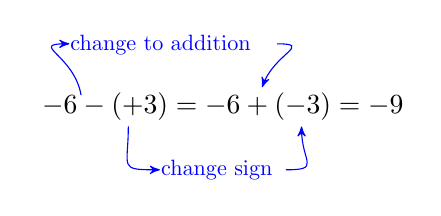
\begin{tikzpicture} 
\coordinate (O) at (0,0);
\node at (O) {$-6-(+3)=-6+(-3)=-9$};
\coordinate(A) at (-1.8,0.15);
\coordinate(B) at (-1.95,.8);
\draw[blue, ->, >=stealth'] (A) to [out=100, in=180, looseness=2, edge node={node[above right, xshift=2, yshift=-3, scale=.8] {change to addition}}] (B);
\coordinate(A) at (0.69,0.8);
\coordinate(B) at (0.5,.25);
\draw[blue, ->, >=stealth'] (A) to [out=0, in=70, looseness=2] (B);
\coordinate(A) at (-1.2,-0.25);
\coordinate(B) at (-0.8,-.8);
\draw[blue, ->, >=stealth'] (A) to [out=270, in=180, looseness=2, edge node={node[below right, xshift=9, yshift=4, scale=.8] {change sign}}] (B);
\coordinate(A) at (.8,-0.8);
\coordinate(B) at (1,-.25);
\draw[blue, ->, >=stealth'] (A) to [out=0, in=270, looseness=2] (B);

\end{tikzpicture}
\newline


fig-2-1-ex4a 2-(-6)

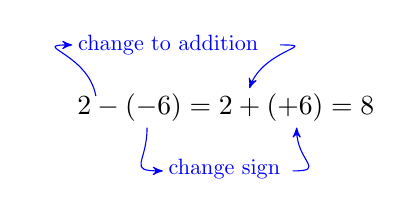
\begin{tikzpicture} 
\coordinate (O) at (0,0);
\node at (O) {$2 -(-6)=2+(+6)=8$};
\coordinate(A) at (-1.65,0.15);
\coordinate(B) at (-1.95,.8);
\draw[blue, ->, >=stealth'] (A) to [out=100, in=180, looseness=2, edge node={node[above right, xshift=2, yshift=-3, scale=.8] {change to addition}}] (B);
\coordinate(A) at (0.69,0.8);
\coordinate(B) at (0.3,.25);
\draw[blue, ->, >=stealth'] (A) to [out=0, in=70, looseness=2] (B);
\coordinate(A) at (-1,-0.25);
\coordinate(B) at (-0.8,-.8);
\draw[blue, ->, >=stealth'] (A) to [out=270, in=180, looseness=2, edge node={node[below right, xshift=7, yshift=4, scale=.8] {change sign}}] (B);
\coordinate(A) at (.85,-0.8);
\coordinate(B) at (.9,-.25);
\draw[blue, ->, >=stealth'] (A) to [out=0, in=270, looseness=2] (B);


\end{tikzpicture}
\newline


fig-2-1-ex4d -7-(-4)

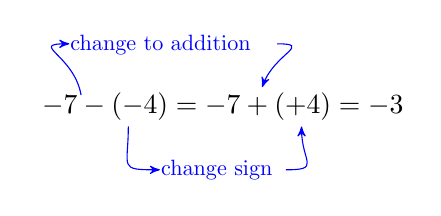
\begin{tikzpicture} 
\coordinate (O) at (0,0);
\node at (O) {$-7-(-4)=-7+(+4)=-3$};
\coordinate(A) at (-1.8,0.15);
\coordinate(B) at (-1.95,.8);
\draw[blue, ->, >=stealth'] (A) to [out=100, in=180, looseness=2, edge node={node[above right, xshift=2, yshift=-3, scale=.8] {change to addition}}] (B);
\coordinate(A) at (0.69,0.8);
\coordinate(B) at (0.5,.25);
\draw[blue, ->, >=stealth'] (A) to [out=0, in=70, looseness=2] (B);
\coordinate(A) at (-1.2,-0.25);
\coordinate(B) at (-0.8,-.8);
\draw[blue, ->, >=stealth'] (A) to [out=270, in=180, looseness=2, edge node={node[below right, xshift=9, yshift=4, scale=.8] {change sign}}] (B);
\coordinate(A) at (.8,-0.8);
\coordinate(B) at (1,-.25);
\draw[blue, ->, >=stealth'] (A) to [out=0, in=270, looseness=2] (B);

\end{tikzpicture}
\newline



sw-2-1-1 number line

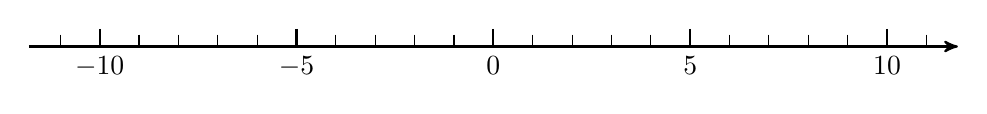
\begin{tikzpicture} [scale=0.5]
\draw[black,thick,->,>=stealth'] (-11.8,0) -- (11.8,0);
\foreach \x in  {-11, -10,...,11} {
 \draw[black] (\x,0.3) --++(0,-0.3);
}
\foreach \x in  {-10, -5, ..., 10} {
 \draw[black, thick] (\x,.45) --++(0,-0.45)  node[below]   {$\x$};
}
\end{tikzpicture}
\newline



sw-2-1-1ans number line

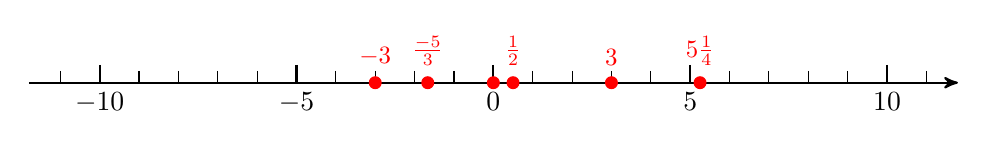
\begin{tikzpicture} [scale=0.5]
\draw[black,thick,->,>=stealth'] (-11.8,0) -- (11.8,0);
\foreach \x in  {-11, -10,...,11} {
 \draw[black] (\x,0.3) --++(0,-0.3);
}
\foreach \x in  {-10, -5, ..., 10} {
 \draw[black, thick] (\x,.45) --++(0,-0.45)  node[below]   {$\x$};
}
\foreach \x in {-3,3} {
 \filldraw[red] (\x,0) circle (.15) node[above, yshift=3, scale=.9] {$\x$};
}
\filldraw[red] (1/2,0) circle (.15) node[above, yshift=3, scale=.9] {$\frac{1}{2}$}; 
\filldraw[red] (-5/3,0) circle (.15) node[above, yshift=3, scale=.9] {$\frac{-5}{3}$}; 
 \filldraw[red] (0,0) circle (.15);
\filldraw[red] (21/4,0) circle (.15) node[above, yshift=3, scale=.9] {$5\frac{1}{4}$};
 \end{tikzpicture}
\newline



sw-2-1-2ans number line

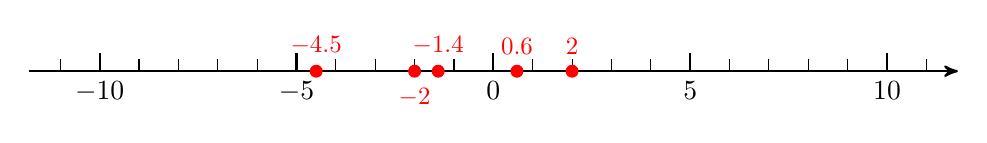
\begin{tikzpicture} [scale=0.5]
\draw[black,thick,->,>=stealth'] (-11.8,0) -- (11.8,0);
\foreach \x in  {-11, -10,...,11} {
 \draw[black] (\x,0.3) --++(0,-0.3);
}
\foreach \x in  {-10, -5, ..., 10} {
 \draw[black, thick] (\x,.45) --++(0,-0.45)  node[below]   {$\x$};
}
\foreach \x in {-4.5,-1.4, 0.6, 2} {
 \filldraw[red] (\x,0) circle (.15) node[above, yshift=3, scale=.9] {$\x$};
}
\filldraw[red] (-2,0) circle (.15) node[below, yshift=-3, scale=.9] {$-2$};
\end{tikzpicture}
\newline


hp-2-2-25 rectangle

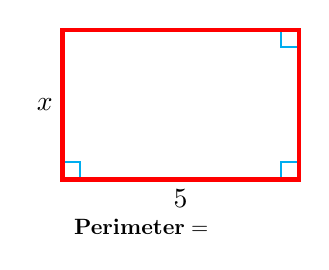
\begin{tikzpicture} 
\coordinate(O) at (0,0);
\coordinate(A) at (3,1.9);
\draw[cyan,thick] (O) rectangle ++(.22,.22);
\draw[cyan,thick] (3,0) rectangle ++(-.22,.22);
\draw[cyan,thick] (A) rectangle ++(-.22,-.22);
\draw[red, ultra thick] (O) rectangle (A);
\node[below] at (1.5,0) {$5$};
\node[below, scale=.8] at (1.,-.4) {$\textbf{Perimeter}=$};
\node[left] at (0,.95) {$x$};
\end{tikzpicture}
\newline


hp-2-2-26 rectangles

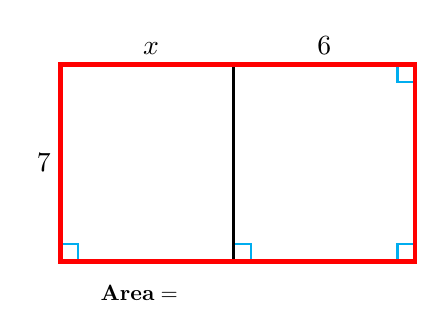
\begin{tikzpicture} 
\coordinate(O) at (0,0);
\coordinate(A) at (4.5,2.5);
\coordinate(B) at (2.2,0);
\draw[cyan,thick] (O) rectangle ++(.22,.22);
\draw[cyan,thick] (B) rectangle ++(.22,.22);
\draw[cyan,thick] (A) rectangle ++(-.22,-.22);
\draw[cyan,thick] (4.5,0) rectangle ++(-.22,.22);
\draw[black, very thick] (B) --++(0,2.5);
\draw[red, ultra thick] (O) rectangle (A);
\node[below, scale=.8] at (1.,-.2) {$\textbf{Area}=$};
\node[left] at (0,1.25) {$7$};
\node[above] at (1.15,2.5) {$x$};
\node[above] at (3.35,2.5) {$6$};
\end{tikzpicture}
\newline




\end{document}
